%\documentclass[trans]{beamer}
\documentclass[10pt]{beamer}

% Try the class options [notes], [notes=only], [trans], [handout],
% [red], [compress], [draft], [class=article] and see what happens!

% Copyright 2003 by Till Tantau <tantau@users.sourceforge.net>.
%
% This program can be redistributed and/or modified under the terms
% of the LaTeX Project Public License Distributed from CTAN
% archives in directory macros/latex/base/lppl.txt.

% For a green structure color use:
%\colorlet{structure}{green!50!black}

%%%%%%%%%% User macros%%%%%%%%%%%
\newcommand{\mypurple}[1]{{\color[rgb]{0.7,0,0.8}#1}}
\newcommand{\myred}  [1] {{\color{red}#1}}
\newcommand{\myblue} [1] {{\color{blue}#1}}
\newcommand{\mygreen}[1] {{\color[rgb]{0,0.5,0}#1}}
\newcommand{\Nat}{\mathbb{N}}
\def\sla  {\!\!\!\slash}
%%%%%%%%%%%%%%%%%%%%%%%%%%%%%%%%%
\mode<article> % only for the article version
{
  \usepackage{beamerbasearticle}
  \usepackage{fullpage}
  \usepackage{hyperref}
}

%\beamertemplateshadingbackground{red!10}{blue!10}
%\beamertemplateshadingbackground{blue!10}{blue!10}

%\usepackage{beamerthemeshadow}

\usepackage{pgf,pgfarrows,pgfnodes,pgfautomata,pgfheaps,pgfshade}
\usepackage{amsmath,amssymb}
\usepackage[latin1]{inputenc}
\usepackage{colortbl}
\usepackage[english]{babel}
%\usepackage{verbatim}
%\usepackage{listings}
\usepackage[procnames]{listings}

%\usepackage{lmodern}
\usepackage[T1]{fontenc} 

\usepackage{times}

% for code colouring
\include{pythonlisting}
\include{cpplisting}
\usepackage{minted}

% Use some nice templates
\beamertemplatetransparentcovereddynamic
\usetheme{Binet}
%\usetheme{Madrid}
%\usetheme{Boadilla}
%\usetheme{Berkeley}
%\usetheme{Rochester}

%\def\command#1{\list{}{\leftmargin=2em\itemindent-\leftmargin\def\makelabel##1{\hss##1}}%
%\item\extractcommand#1@\par\topsep=0pt}
%\def\endcommand{\endlist}
%\def\extractcommand#1#2@{\strut\declare{\texttt{\string#1}}#2}

%
% The following info should normally be given in you main file:
%

\hypersetup{%
  pdftitle={Core s/w in \texttt{LHCb}},%
  pdfauthor={Sebastien Binet}
  %pdfsubject={AthenaMP},
  %pdfkeywords={ATLAS,Athena,python,COW,parallelization},
%  pdfpagemode=FullScreen%
}

\title[core s/w]{Core s/w in \texttt{LHCb}}
\author[S. Binet]{S\'ebastien~Binet}%\inst{1}
\institute[LAL]{
%  \inst{1}%
  LAL/IN2P3}
\date{2014-03-11}

% \begin{center}
% On behalf of Core people
% \end{center}

\pgfdeclaremask{lal}{lal}
%\pgfdeclaremask{ubp}{UBP-logo}
\pgfdeclareimage[mask=lal,width=2cm]{lal-logo}{lal}
%\pgfdeclareimage[mask=ubp,width=1cm]{ubp-logo}{UBP-logo}

\logo{%
  \vbox{%
    \hbox{\pgfuseimage{lal-logo}}%
  }%
}


\begin{document}
\lstset{language=C++}

\frame{\titlepage
%  \hskip0.44\paperwidth
%  \insertlogo

    \begin{beamercolorbox}[sep=8pt,center]{mylogo}
      \usebeamercolor{mylogo}\insertlogo
    \end{beamercolorbox}

}

%\section*{Outline}
%\frame{\tableofcontents[part=1]}%,pausesections]}

%\AtBeginSubsection[]
%{
%  \frame<handout:0>
%  {
%    \frametitle{Outline}
%    \tableofcontents[current,currentsubsection]
%  }
%}

\part<presentation>{Main Talk}

%%%%%%%%%%%%%%%%%%%%%%%%%%%%%%%%%%%%%%%%%%%%%%%%%%%%%%%%%%%%%%%%%%%%%%%%%%%%%%%
%%%%%%%%%%%%%%%%%%%%%%%%%%%%%%%%%%%%%%%%%%%%%%%%%%%%%%%%%%%%%%%%%%%%%%%%%%%%%%%
%\section[Outline]{Outline}

% \frame<beamer>{
%   \frametitle{Outline}
%   \begin{columns}
% \begin{column}{0.49\textwidth}
%   \begin{block}{}
%   \tableofcontents
%   \end{block}
% \end{column}
% \end{columns}

% }
%\frame{\partpage}

%%%%%%%%%%%%%%%%%%%%%%%%%%%%%%%%%%%%%%%%%%%%%%%%%%%%%%%%%%%%%%%%%%%%%%%%%%%%%%%
%%%%%%%%%%%%%%%%%%%%%%%%%%%%%%%%%%%%%%%%%%%%%%%%%%%%%%%%%%%%%%%%%%%%%%%%%%%%%%%
\section[mysection]{mysection}

\frame{
  \frametitle{Introduction}

  \begin{exampleblock}{}
    Most of \texttt{core s/w} work happens in \texttt{Gaudi} \\(at
    least, the one I am interested in and paid for)
  \end{exampleblock}

  \begin{block}{}
    \texttt{Gaudi} is:
    \begin{itemize}
      \item a component object model (\texttt{COM}) based framework
      \item mainly written in \texttt{C++}
      \item with bits and pieces written in \texttt{python} for
        steering
      \item (although more and more pieces in \texttt{python} for
        analysis)
        \begin{itemize}
          \item similar situation in \texttt{ATLAS}
        \end{itemize}
      \item most of the code written under a \emph{single thread}
        assumption
        \begin{itemize}
          \item most of the code is \mypurple{not thread safe}
        \end{itemize}
    \end{itemize}
  \end{block}
}

\frame{
  \frametitle{\texttt{Gaudi} refresher}

  \begin{columns}
    \begin{column}{0.25\textwidth}
      \begin{block}{}
        \begin{itemize}
          \item application mgr
          \item event processor
          \item algorithms
          \item data store
          \item component object model
          \item single thread
        \end{itemize}
      \end{block}
    \end{column}

    \begin{column}{0.75\textwidth}
      \includegraphics[width=1\linewidth]{figs/athena-component-model.pdf}
    \end{column}
  \end{columns}
}

\begin{frame}[fragile]
\frametitle{\texttt{Gaudi} refresher - II}

  \begin{center}
    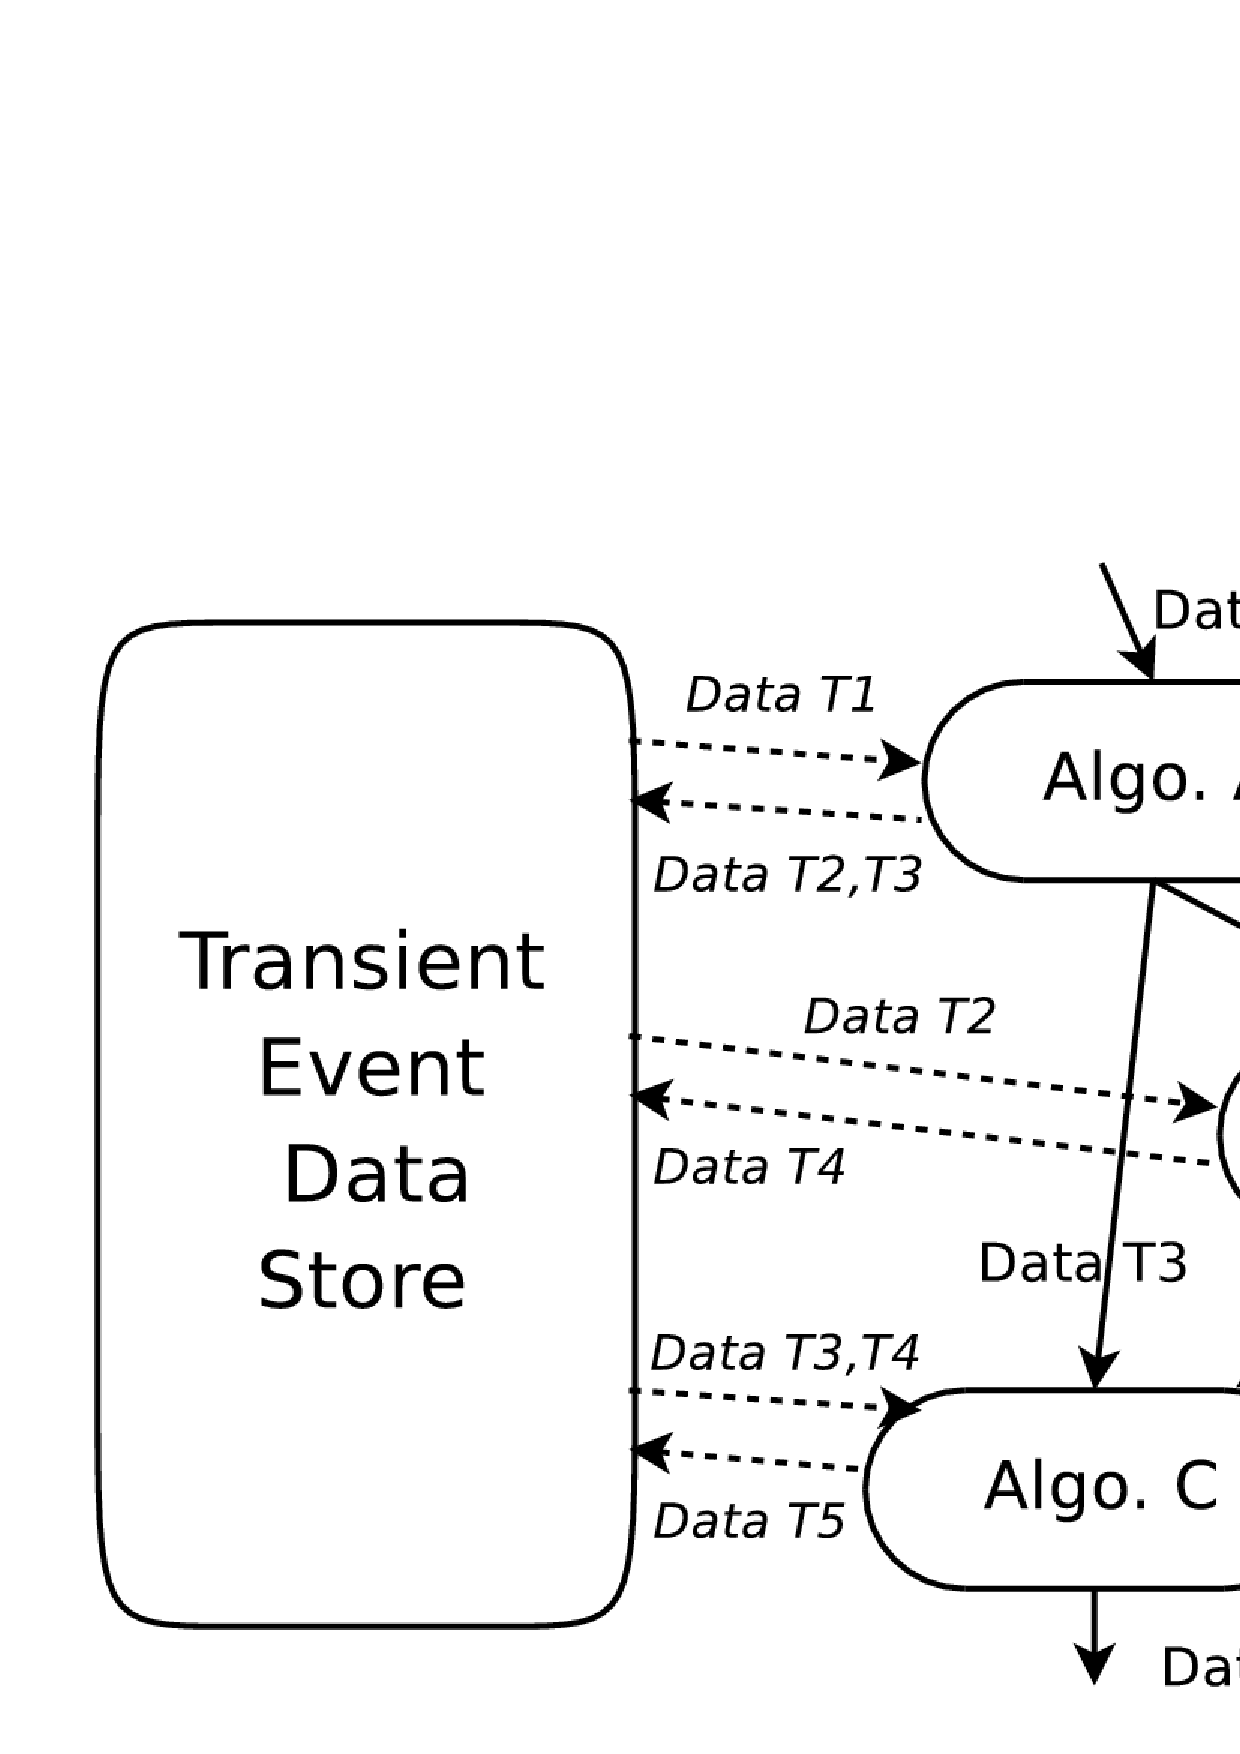
\includegraphics[width=0.6\linewidth]{figs/storegatesvc.pdf}

\begin{minted}[]{c++}
class IAlgorithm { public:
  virtual StatusCode initialize() = 0;
  virtual StatusCode execute() = 0;
  virtual StatusCode finalize() = 0;
};
\end{minted}
  \end{center}

\end{frame}


\frame{
  \frametitle{Motivations: hardware trends}
  \begin{block}{}
        \begin{itemize}
          \item \emph{CPU} $\Rightarrow$ multicores
          \item large number of \emph{CPU} cores calls for more parallelism
            \begin{itemize}
              \item event parallelism inherent to typical \emph{HEP} selection and reconstruction programs
              \item parallelization inside applications may provide huge speed ups but requires typically also careful (re)design of code
            \end{itemize}
          \item exploit parallelism with:
            \begin{itemize}
              \item multi-threading (\texttt{GaudiMT/GaudiHive})
              \item multi-processes (\texttt{GaudiMP/GaudiParallel})
            \end{itemize}
        \end{itemize}
  \end{block}
}

\frame{
  \frametitle{Motivations: boundary conditions (\texttt{Run-I})}
      \begin{block}{}
        \begin{itemize}
          \item \texttt{LHCb} has large code basis mostly written and designed in \emph{``pre-multi-core era''}
            \begin{itemize}
              \item \emph{online} and \emph{offline} reconstruction code mainly process based and single threaded
            \end{itemize}
          \item experimented with multi-threading and multi-processes:
            \begin{itemize}
              \item existing code basis implies boundary conditions for future developments
              \item modifications have to be as transparent as possible
            \end{itemize}
        \end{itemize}
      \end{block}
}

\frame{
  \frametitle{Multi-threading: \texttt{GaudiMT}}

  \begin{columns}
    \begin{column}{0.9\textwidth}
      \begin{block}{}
        \begin{itemize}
          \item Code sharing
          \item Small context switch times $\rightarrow$ \emph{``lightweight processes''}
          \item Automatic sharing of many hardware resources
        \end{itemize}
      \end{block}
    \end{column}
  \end{columns}

  \begin{columns}
    \begin{column}{0.7\textwidth}
      \begin{exampleblock}{}
        \begin{itemize}
        \item Event processing in multiple worker threads
        \item HLT selection software controlled by TDAQ framework
        \item Special version of \texttt{Gaudi/Athena} framework to create selection algorithm instances for worker threads
        \item Development and \emph{MT} tests started on dual
          processor single core machines, long before multi-core
          machines were available (\texttt{Atlas})
        \end{itemize}
        \end{exampleblock}
    \end{column}

    \begin{column}{0.3\textwidth}
      \begin{figure}
        \begin{center}
          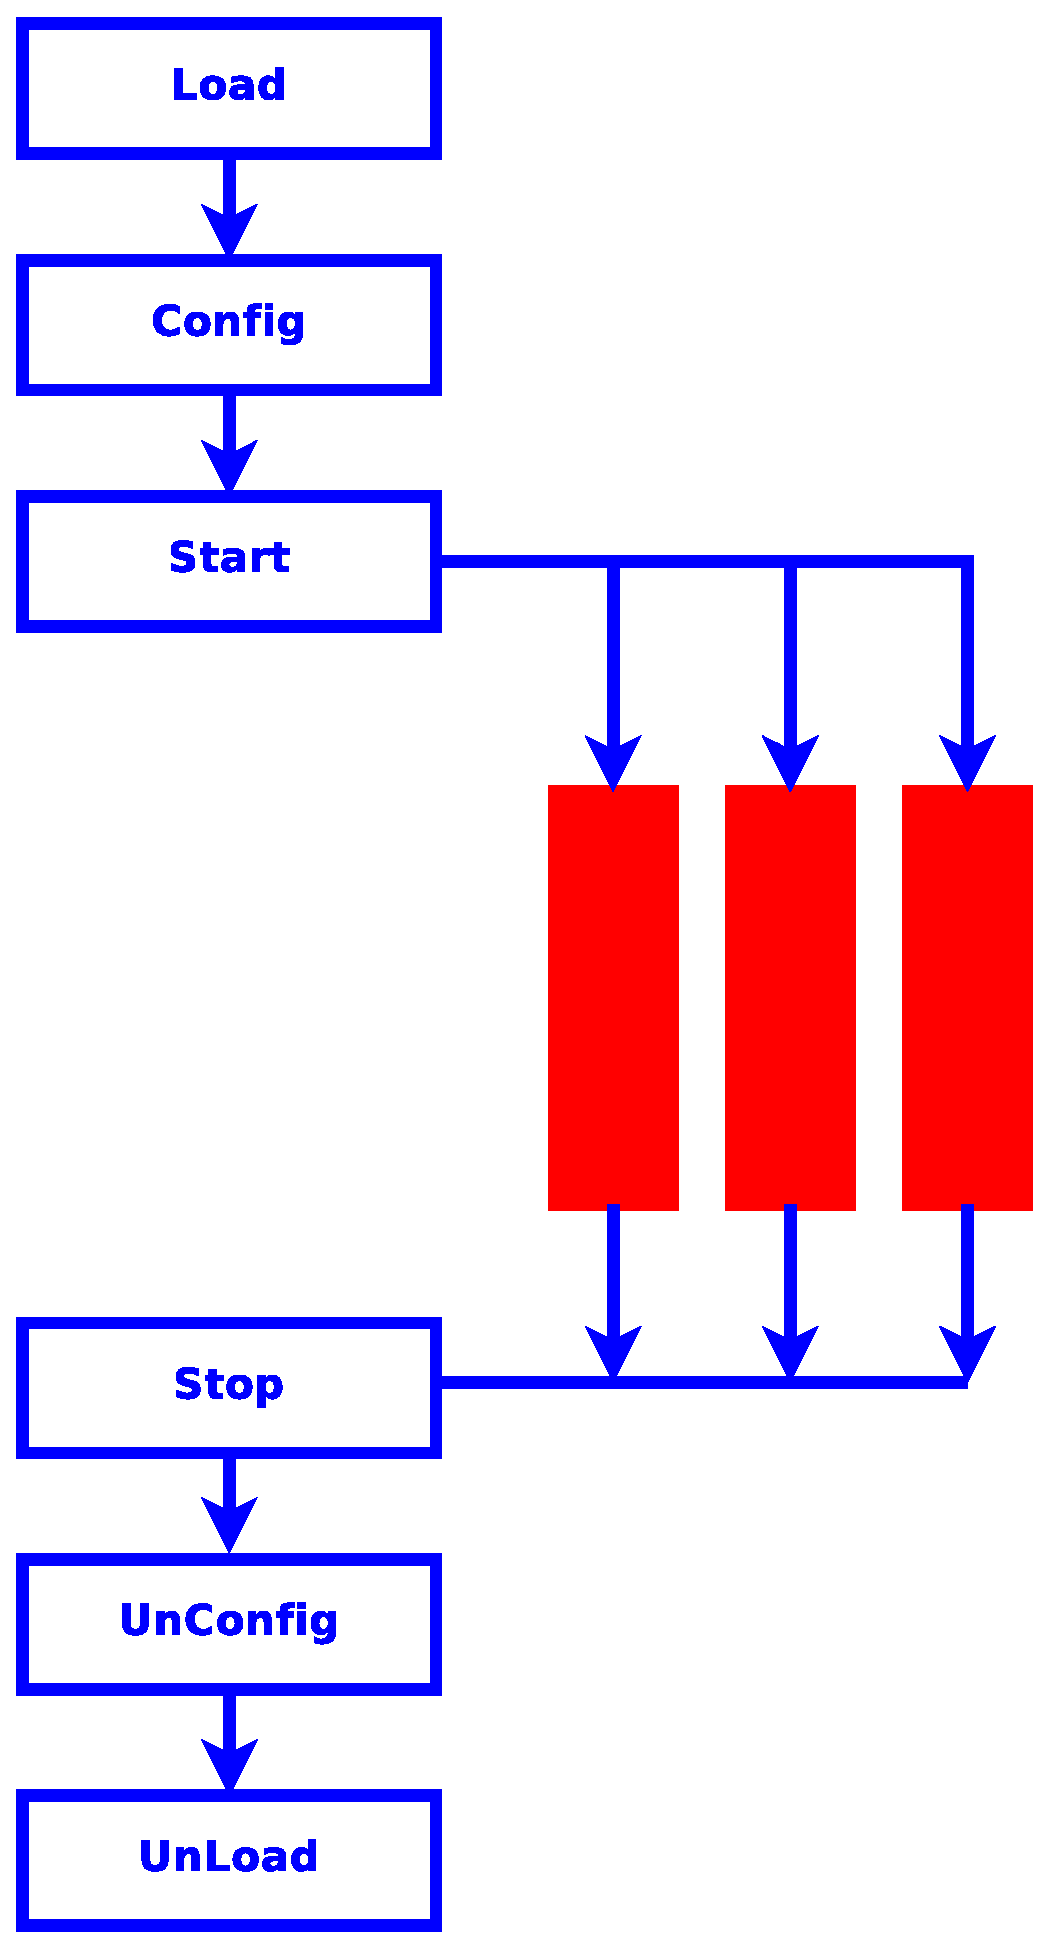
\includegraphics[angle=0,width=0.8\textwidth]{figs/tdaq-mt-flow.eps}
        \end{center}
      \end{figure}
    \end{column}
  \end{columns}
}

\frame{
  \frametitle{Multi-threading support in \texttt{Gaudi} framework}

%  \begin{columns}
%    \begin{column}{0.9\textwidth}
%      \begin{block}{}
        \begin{itemize}
          \item \myred{Multi-threading:} all services and algorithms which modify data have to be thread specific (\emph{e.g.} \texttt{StoreGate/EventStore})
            \begin{itemize}
              \item threads may however also use \mypurple{``read only''} services which are common to all threads (\emph{e.g.} \texttt{GeometrySvc, DetectorStore})
            \end{itemize}
          \item all thread-specific instances of services and algorithms are distinguished by \myred{type} and \myred{\texttt{(generic name)\_\_(thread ID)}}
            \begin{itemize}
              \item \emph{e.g.} create an algorithm of type \mygreen{\texttt{TriggerSteering}} and generic name \mygreen{\texttt{TrigStr}} for 2 threads:
                \begin{itemize}
                  \item \mygreen{\texttt{TriggerSteering/TrigStr\_\_0}}
                  \item \mygreen{\texttt{TriggerSteering/TrigStr\_\_1}}
                \end{itemize}
            \end{itemize}
          \item Assumption:
            \begin{itemize}
              \item \myred{Algorithms} are \mypurple{always thread specific}
                \begin{itemize}
                  \item for each thread an algorithm copy is generated automatically
                \end{itemize}
              \item if a \myred{Service} is run thread specific or common for all threads has to be specified in the configuration
            \end{itemize}
          \item modified \texttt{Gaudi/Athena} can also be used for normal offline running
        \end{itemize}
%      \end{block}
%    \end{column}
%  \end{columns}

}

\frame{
\frametitle{Experiences with multi-threading}
\begin{block}{}
  \begin{itemize}
    \item created different event selection slices which could run multithreaded
    \item some technical issues are historical now but interesting:
      \begin{itemize}
        \item implementation of \texttt{STL} elements with different compiler versions
          \begin{itemize}
            \item memory allocation model not optimal for \emph{``event parallelism''}
          \end{itemize}
        \item thread safe external libraries
      \end{itemize}
  \end{itemize}
\end{block}

}

\frame{
\frametitle{Experiences with multi-threading - II}
\begin{exampleblock}{Software development}
  \begin{itemize}
    \item developers have to be familiar with thread programming
      \begin{itemize}
        \item need special training and knowledge
      \end{itemize}
    \item developers have to take into account for their code the MT model of L2 $\Rightarrow$ \mypurple{event parallelism}
    \item synchronization problems for multi-threaded code are tedious to debug
    \item need good tools to assist developers for debugging and optimizing multi-threaded programs
    \item typically selection code \mypurple{changes rapidly} due to physics needs
      \begin{itemize}
        \item \myred{constant need for re-optimization}
      \end{itemize}
  \end{itemize}
\end{exampleblock}

\begin{alertblock}{}
  \begin{itemize}
    \item \myred{Problem:} preserve thread safe and optimized code over release cycles and in a large heterogeneous developer community
      \begin{itemize}
        \item coupling of different sw communities with different goals
      \end{itemize}
  \end{itemize}
\end{alertblock}
\small{
Presently we (\texttt{Atlas}) run $n$ ($= \# cores$) instances of L2  Processing Unit on a multi-core machine with one worker thread}
}

\frame{
  \frametitle{\texttt{Process-based parallelism}}

  \begin{columns}
    \begin{column}{0.9\textwidth}
      \begin{exampleblock}{}
        \begin{itemize}
          \item run $n$ process instances on machine with $n$ cores
            \begin{itemize}
              \item easy to do with existing code
              \item \emph{a priori} no code changes required
              \item observe good scaling with number of cores
            \end{itemize}
        \end{itemize}
      \end{exampleblock}

      \begin{block}{Problem(s)}
        \begin{itemize}
          \item resource sharing and optimization
          \item resource requirements are multiplied w/ nbr of process instances
          \item \myred{memory size}
          \item OS resources: file descriptors, network sockets, \ldots
          \item on trigger farms:
            \begin{itemize}
              \item number of controlled applications
              \item number of network connections to readout system
              \item transfer of same configuration data $n$ times to the same machine
              \item recalculation of the same configuration data $n$ times
              \item optimal \emph{CPU} utilization: use \emph{CPU} for event processing while waiting for input data
            \end{itemize}
        \end{itemize}
      \end{block}

    \end{column}
  \end{columns}
}

\frame{
  \frametitle{Memory sharing via \texttt{fork}}
  \begin{itemize}
    \item Basic idea:
      \begin{itemize}
        \item run multiple reconstruction jobs, sharing as much memory as possible
        \item minimize number of required code changes
          \begin{itemize}
            \item let the \texttt{OS} do most of the work
          \end{itemize}
        \item use {\bf\myred{\texttt{fork()}}}
      \end{itemize}
    \item \texttt{fork()}:
      \begin{itemize}
        \item \texttt{fork()} clones a process, including its entire address space
        \item modern OS' \texttt{fork()} uses \mypurple{\emph{``Copy On Write''}}
          \begin{itemize}
            \item memory is shared up to the point a process writes to it
            \item memory will be copied and the affected changes will become unshared
          \end{itemize}
        \item \texttt{fork()} as late as possible but before any output is written
        \item as much memory as possible is \mypurple{automatically shared} between processes
          \begin{itemize}
            \item memory which is modified will become unshared
            \item static configuration data will remain shared
          \end{itemize}
      \end{itemize}
  \end{itemize}
}

\frame{
  \frametitle{Memory sharing via \texttt{fork} - II}
\begin{block}{}
\begin{itemize}
  \item advantages:
    \begin{itemize}
      \item \mypurple{all} memory that can be shared \mypurple{will be}
      \item code changes restricted to few framework packages, bulk of the code remains untouched
      \item don't need to worry about \mygreen{locking}
    \end{itemize}
\end{itemize}
\end{block}

\begin{exampleblock}{}
  \begin{itemize}
    \item disadvantages
      \begin{itemize}
        \item memory can not be \mypurple{re-shared} after it became unshared
          \begin{itemize}
            \item maybe a problem for conditions data
          \end{itemize}
      \end{itemize}
  \end{itemize}
\end{exampleblock}

\begin{figure}
  \begin{center}
    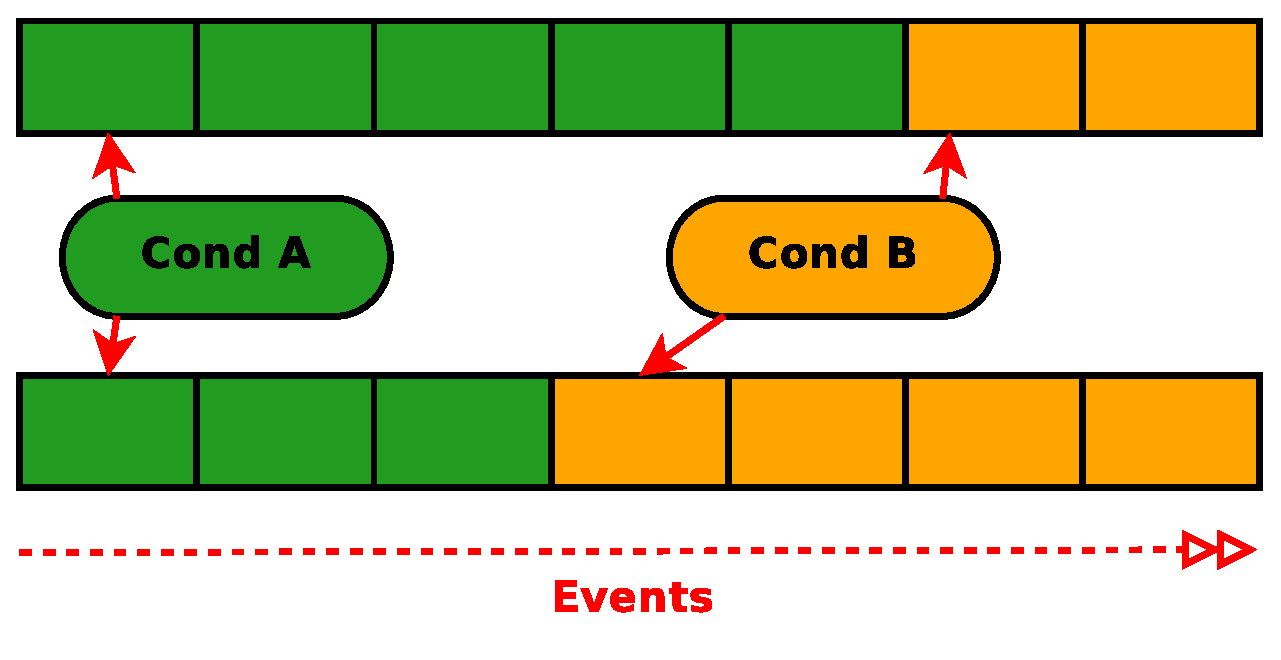
\includegraphics[angle=0,width=0.65\textwidth]{figs/cond-data-flow.eps}
  \end{center}
\end{figure}
}

\frame{
  \frametitle{\texttt{GaudiMP} implementation}

  \begin{columns}
    \begin{column}{0.95\textwidth}

      \begin{block}{}
        \begin{itemize}
          \item avoid clients' changes
          \item hide MP-semantics \myred{inside} \texttt{Gaudi} instead of publishing them as a layer on top
          \item use the \texttt{python} module
            \mygreen{\texttt{multiprocessing}} (backported from 2.6)
            for the process management (\mypurple{now, a proper
              \texttt{C++} component})
          \item write a new event loop manager as a usual \texttt{Gaudi} component to encapsulate the parallelism handling
          \item modify the I/O-related components appropriately
        \end{itemize}
      \end{block}

    \end{column}
  \end{columns}

\begin{figure}
  \begin{center}
    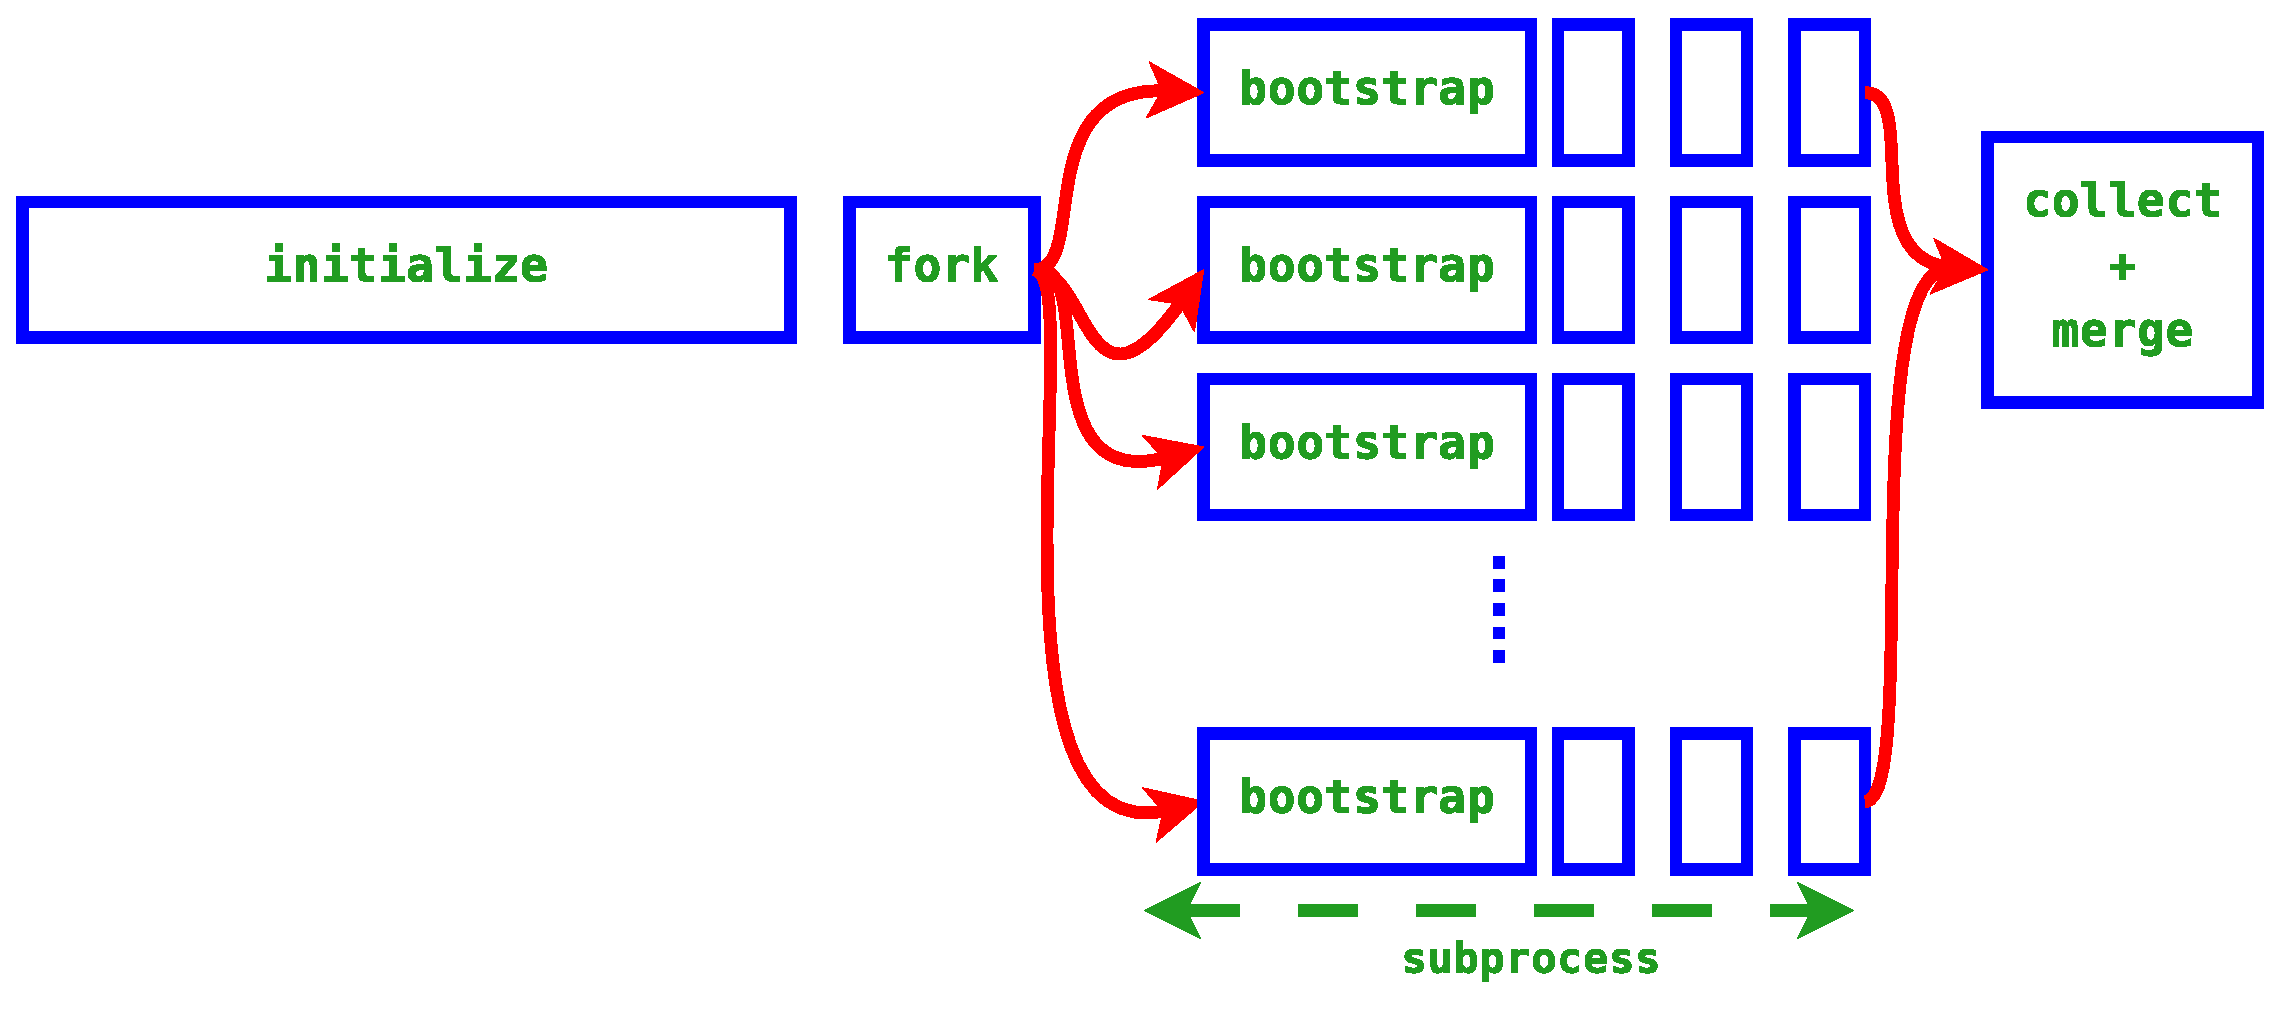
\includegraphics[angle=0,width=0.7\textwidth]{figs/athenamp-sequence.eps}
  \end{center}
\end{figure}
}

\frame{
  \frametitle{Experiences with multi-processes}
\begin{block}{}
  \begin{itemize}
    \item limited long range impact
    \item modifications applied to control framework and I/O-related components
    \item easier to develop with
      \begin{itemize}
        \item no implicit sharing
        \item no lock, races, \ldots
      \end{itemize}
  \end{itemize}
\end{block}

\begin{alertblock}{Problems}
  \begin{itemize}
    \item random numbers, seeds and reproducibility
    \item I/O
      \begin{itemize}
        \item need to chase people directly \texttt{open()}ing files, by-passing framework hooks
        \item merging output files is tedious (but needed for production)
      \end{itemize}
    \item GRID
      \begin{itemize}
        \item submission of MP-jobs (overbooking computing nodes)
        \item \texttt{vmem} accounting
          \begin{itemize}
            \item most of grid resource monitoring tools will double-count the memory shared by \texttt{fork()}ed subprocesses
          \end{itemize}
      \end{itemize}
  \end{itemize}
\end{alertblock}
}

\frame{
  \frametitle{(first) Conclusions}

\begin{exampleblock}{}
  \begin{center}
    It is possible to refactor an already existing
    \texttt{FORTRAN/C/C++} application, written in a
    \emph{single-threaded} fashion (like \texttt{Gaudi}) with minimal
    modifications (or at least \myred{localised}) to better leverage
    the \emph{new} multicore architectures.
  \end{center}
\end{exampleblock}

\begin{alertblock}{}
Automa(g)ic \emph{scaling} with the number of cores ?
\begin{itemize}
 \item unlikely if $N_{\texttt{cores}} \geq 1024$ (memory resources)
 \item unlikely at the \texttt{I/O} level
 \item \emph{mapping} 1 processus per core \myred{not fine-grained enough}
\end{itemize}
\end{alertblock}

\begin{block}{}
\begin{center}
 \begin{itemize}
  \item \myred{concurrency} at the \mypurple{event} level
  \item \myred{concurrency} at the \mypurple{algorithm} level
  \item \myred{concurrency} \mypurple{within the algorithms}
 \end{itemize}

$\Rightarrow$ \myred{multithreading !}\\
$\Rightarrow$ \myred{\texttt{GaudiHive project}}
\end{center}
\end{block}
}

\frame{
  \frametitle{Concurrency in \verb~HEP~ frameworks}
New developments and/or adiabatic evolution of \texttt{Gaudi} need to:

\begin{itemize}
\item prepare for further \alert{gains} by exploiting features of today's CPUs' 
  $\mu$-architecture
\begin{itemize}
\item vector registers, instruction pipelining, multiple instructions per cycle
    (see Sverre Jarp presentations at CHEP)
\item improve data and code locality, hardware threading
\item (also relevant for non-fwk code)
\end{itemize}
\item prepare for, or at least don't prevent use of, 
  \alert{off-loading large computations} to accelerators (GPGPUS, Xeon Phi)
\item prepare for increased exposed concurrency
\begin{itemize}
\item a means for better memory usage and improved throughput
\end{itemize}
\end{itemize}
}

\frame{
\frametitle{Concurrency in \verb~HEP~ frameworks - II}
\begin{center}
\includegraphics[width=0.66\linewidth]{figs/conc-level.pdf}
\end{center}
}

\begin{frame}[fragile]
\frametitle{Concurrency in \verb~HEP~ frameworks - III}
\label{sec-1-5}


Various levels of concurrency can be exposed in current \verb~HEP~ applications:

\begin{itemize}
\item \alert{event-level} concurrency
\begin{itemize}
\item the framework allows to properly and safely process multiple events
    at a given time
\end{itemize}
\item \alert{algorithm-level} concurrency, \alert{task-} and/or \alert{data-} oriented concurrency
\begin{itemize}
\item the framework allows to partition the processing of an event into various
    sub-tasks (calorimetry, tracking, RoIs, \ldots{})
\item \alert{task/functional} oriented concurrency: split according to ``logical'' tasks
\item \alert{data} oriented concurrency: partition the data domain
\end{itemize}
\item \alert{subalgorithm-level} concurrency
\begin{itemize}
\item each algorithm can itself exposes concurrent sub-sub-tasks
\item leverage co-processors, vector units, \ldots{}
\end{itemize}
\end{itemize}
\end{frame}

\begin{frame}[fragile]
\frametitle{Concurrency in \verb~HEP~ frameworks - IV}
\label{sec-1-6}


\alert{Event-level} concurrency is achieved by:

\begin{itemize}
\item modifying the event loop to hand over multiple events
\item put these multiple events into multiple event stores
\item have algorithms and sequence of algorithms work on these stores
\end{itemize}

\alert{REQUIRES} that at least the core components are \alert{race-free} and \alert{thread-safe}
\end{frame}
\begin{frame}[fragile]
\frametitle{Concurrency in \verb~HEP~ frameworks - V}
\label{sec-1-7}


\alert{Alg-level} concurrency is achieved by:

\begin{itemize}
\item modifying the algorithm manager to execute multiple algorithms concurrently
\item \alert{need} new information to properly schedule these algorithms in the correct
  order: \alert{data dependency graph} (hopefully acyclic!)
\begin{itemize}
\item either extracted at \alert{runtime} during a warm-up
    phase or \alert{explicitly} at \alert{configuration-time}
\end{itemize}
\end{itemize}

\begin{figure}
  \begin{center}
    \includegraphics[width=0.45\textwidth]{figs/data-flow.pdf}
    \includegraphics[width=0.45\textwidth]{figs/gaudi-hive-1.png}
  \end{center}
\end{figure}
\end{frame}
\begin{frame}[fragile]
\frametitle{Concurrency in \verb~HEP~ frameworks - VI}
\label{sec-1-8}


\alert{SubAlg-level} concurrency is achieved by:

\begin{itemize}
\item providing tools or libraries to expose concurrency
\item making the framework aware of the available resources
\item making the framework aware of the different tools/libraries for
  an efficient scheduling
\end{itemize}
\end{frame}

\frame{
  \frametitle{Many concurrent events}
  \begin{columns}
    \begin{column}{0.7\textwidth}
      \begin{block}{}
        \begin{itemize}
          \item Need to deal with the tails of sequential processing
            \begin{itemize}
              \item there is always an \texttt{Algorithm} taking very
                long producing data needed by many others
            \end{itemize}
          \item introducing \texttt{pipeling} processing
            \begin{itemize}
              \item exclusive access to resources
              \item non-reentrant algorithms
              \item \emph{e.g.} file writing, DB access, \ldots
            \end{itemize}

            \item Current frameworks handle a single event at the
              time. They need to be evolved
              \begin{itemize}
                \item design a powerful and flexible
                  \texttt{Algorithm} scheduler
                \item need to define the concept of an \texttt{event context}
              \end{itemize}
        \end{itemize}
      \end{block}
    \end{column}
    \begin{column}{0.3\textwidth}
      \includegraphics[width=1\textwidth]{figs/gaudi-hive-2.png}
    \end{column}
  \end{columns}

}

\frame{
  \frametitle{Example: \texttt{LHCb} reconstruction}

  \includegraphics[width=1\textwidth]{figs/dag-brunel.png}

  \begin{columns}
    \begin{column}{0.65\textwidth}
      \begin{block}{}
        \begin{itemize}
          \item DAG of \texttt{Brunel} (214 \texttt{Algorithm}s)
            \begin{itemize}
              \item obtained by instrumenting the existing sequential
                code
              \item probably still missing 'hidden or indirect' dependencies
            \end{itemize}

            \item this can give us an estimate of the potential for
              \emph{concurrency}
              \begin{itemize}
                \item assuming no changes in current reconstruction algorithms
              \end{itemize}
        \end{itemize}
      \end{block}
    \end{column}
    \begin{column}{0.35\textwidth}
      \includegraphics[width=1\textwidth]{figs/dag-brunel-close-up.png}
    \end{column}
  \end{columns}
  
}

\begin{frame}
\frametitle{Implementation and PoC}
\label{sec-1-9}


Testbed for these developments: \alert{GaudiHive}

  \begin{columns}
    \begin{column}{0.7\textwidth}

      \begin{block}{}
        \begin{itemize}
          \item a LCG/LHCb/ATLAS project
          \item toy framework evolving into a real one
          \begin{itemize}
            \item No real algorithms but CPU crunchers
            \item timing of real workflow reproduced
          \end{itemize}
          \item Schedule algorithm when its inputs are available
        \end{itemize}
      \end{block}

    \end{column}
    \begin{column}{0.35\textwidth}
\begin{figure}
  \begin{center}
    \includegraphics[width=0.95\textwidth]{figs/gaudi-hive.png}
  \end{center}
\end{figure}
    \end{column}
  \end{columns}
\end{frame}
\begin{frame}
\frametitle{Implementation and PoC - II}
\label{sec-1-10}


  \begin{columns}
    \begin{column}{0.7\textwidth}

      \begin{block}{}
        \begin{itemize}
          \item Multiple events managed simultaneously
          \begin{itemize}
             \item bigger probability to schedule an alg
             \item whiteboard integrated in the \texttt{DataSvc}
             \item \texttt{DataSvc} made thread-safe
          \end{itemize}
          \item Several copies of the same algorithms can coexist
          \begin{itemize}
             \item running on different events
             \item responsibility of \texttt{AlgoPool}
          \end{itemize}
          \item Data specific to execution stored in the \emph{execution context}
        \end{itemize}
      \end{block}

    \end{column}
    \begin{column}{0.35\textwidth}
\begin{figure}
  \begin{center}
    \includegraphics[width=0.95\textwidth]{figs/gaudi-hive.png}
  \end{center}
\end{figure}
    \end{column}
  \end{columns}
\end{frame}
\begin{frame}[fragile]
\frametitle{Implementation notes}
\label{sec-1-11}


\begin{itemize}
\item task-oriented concurrency handled via \alert{TBB}
\begin{itemize}
\item \textbf{de facto} standard among experiments (\verb~ATLAS~, \verb~CMS~ and \verb~LHCb~)
\item useful concurrent containers and algorithms (\verb~parallel_for~,\ldots{})
\end{itemize}
\item leverage \verb~C++11~ constructs and memory model
\begin{itemize}
\item atomics
\item confortable syntax (range-based \verb~for~ loops, \verb~auto~, \verb~tuples~)
\end{itemize}
\item new algorithm steering to handle dependency graph
\begin{itemize}
\item \alert{opportunity} to streamline/harmonize with \verb~trigger steering~ solution
\end{itemize}
\item thread-safe message service (\verb~TBBMessageService~)
\item work on a thread-safe \verb~ToolSvc~ and \verb~ServiceMgr~
\item auditors ? incidents ?
\end{itemize}
\end{frame}

\frame{
  \frametitle{Test on \texttt{Brunel} workflow}
  \begin{columns}
    \begin{column}{0.5\textwidth}
      \begin{block}{}
        \begin{itemize}
          \item 214 algorithms, real data dependencies, (average) real
            timing
            \begin{itemize}
              \item maximum speedup depends stringly on the workflow chosen
            \end{itemize}
            \item adding more simultaneous events moves the maximum
              concurrency from 3 to 4 with single \texttt{Algorithm}
              instances
            \item increased parallelism when cloning algorithms
              \begin{itemize}
                \item even with a moderate number of events in flight
              \end{itemize}
        \end{itemize}
      \end{block}
    \end{column}
    \begin{column}{0.5\textwidth}
  \begin{center}
    \includegraphics[width=0.95\textwidth]{figs/brunel-perfs.png}
  \end{center}
  \begin{exampleblock}{}
    Test system with 12 physical cores \\ x2 hyperthreads (HT)
    \end{exampleblock}
    \end{column}
  \end{columns}
}

\frame{
  \frametitle{Concurrent \texttt{Gaudi}: status}
  \begin{block}{}
    \begin{itemize}
      \item a prototype of a concurrent \texttt{Gaudi}
        (\texttt{GaudiHive}) has been developed as an evolution (new
        branch in the \texttt{Gaudi} repository)
        \begin{itemize}
          \item able to schedule and run \mypurple{algorithms
            concurrently}
            \item able to run \mypurple{multiple events
              simultaneously}
            \item friendly with \mypurple{sub-event parallelism} if
              using \texttt{TBB}
        \end{itemize}

      \item so far, tested with \texttt{Brunel} reconstruction
        workflow:
        \begin{itemize}
          \item important speedup already been obtained, but no
            \emph{'perfect'} scaling achieved yet
          \item \texttt{Algorithm} cloning increases parallelism,
            keeps \emph{latency} under control
        \end{itemize}

        \item test bench to exercize timings and dependencies for
          other applications:
          \begin{itemize}
            \item \texttt{CMSSW} reconstruction workflow
            \item \texttt{ATLAS} calo-reconstruction
          \end{itemize}
    \end{itemize}
  \end{block}
}

\frame{
  \frametitle{Conclusions}
  \begin{block}{}
    \begin{itemize}
      \item Applications will increasingly need to be concurrent if we
        want to fully exploit the continuing exponential CPU
        throughput gains
        \begin{itemize}
          \item parallelizing the framework spares physicists from
            developing parallel code and is the natural place to have
            the full overview and control of the application
          \item but physicists will need to be somewhat aware of
            parallelism/concurrency programming to efficiently
            leverage (and code for) sub-event parallelism
        \end{itemize}

      \item Prototype of \texttt{Gaudi} framework with concurrency has
        been developed
        \begin{itemize}
          \item ideal test-bench for validating scheduling strategies
          \item more real tests on the way (LHCb/ATLAS)
        \end{itemize}

      \item a clear trend emerged for the future of HEP data
        processing
        \begin{itemize}
          \item parallelism within the algorithm
          \item parallelism among algorithms
          \item parallelism among events
        \end{itemize}
    \end{itemize}
  \end{block}
}
\end{document}


